\documentclass{article}
\usepackage{../../../settings}

\begin{document}
\hexcover{Py 心寫程式}{學習歷程}{作者：曾嘉禾}{Dandelion}{電算社}

\begin{large}

\begin{boxpar}{Dandelion}{製作說明}
與電算社組員共同以 Python 的 pygame 函式庫開發一款三關卡圖形化遊戲，涵蓋滑鼠操控躲避、鍵盤操控物理模擬，以及點擊反應測試等機制。本人擔任組長，負責統籌開發進度、技術決策與組員協調。
\end{boxpar}

\begin{boxpar}{Dandelion}{動機}
    \begin{itemize}
        \item 受同校學長姐啟發，希望以實際專題驗證自學成果
        \item 有自學 Python、Linux shell script 與 C++ 的背景，認為遊戲開發是整合這些能力的好機會
        \item 希望透過團隊合作體驗真實軟體開發流程，而非單打獨鬥
    \end{itemize}
\end{boxpar}

\begin{boxpar}{Dandelion}{技術決策：引擎選擇}
開發初期面臨 Godot 與 pygame 的選擇，進行了系統性比較。

\begin{itemize}
    \item \textbf{Godot} 具備圖形化介面與 3D 支援，但強度依賴專屬編輯器，學習成果難以遷移至其他開發場景
    \item \textbf{pygame} 是純 Python 函式庫，學習過程等同深化 Python 能力，不受限於特定工具鏈，可在任何編輯器中開發
\end{itemize}

最終選擇 pygame，核心考量是工具的可遷移性比功能的豐富性更重要。
\end{boxpar}

\begin{boxpar}{Dandelion}{遊戲關卡}
    \begin{boxpar}{Dandelion}{第一關：躲避隕石（滑鼠操控）}
        \begin{itemize}
            \item 玩家以滑鼠操控角色躲避四面而來的隕石
        \end{itemize}
    \end{boxpar}
    \begin{boxpar}{Dandelion}{第二關：躲避隕石（鍵盤與物理模擬）}
        \begin{itemize}
            \item 玩家以鍵盤左右移動
            \item 隕石以重力加速度向下掉落，模擬真實物理行為
        \end{itemize}
    \end{boxpar}
    \begin{boxpar}{Dandelion}{第三關：打淑麗（非原創）}
        \begin{itemize}
            \item 以附中校長為題材的點擊反應遊戲
            \item 正確點擊得分，點錯觸發延遲懲罰機制
        \end{itemize}
    \end{boxpar}
\end{boxpar}

\begin{boxpar}{Dandelion}{開發過程中的問題與解決}
\begin{itemize}
    \item \textbf{pygame.display 的 FPS 與計時器管理}
        \begin{itemize}
            \item 電腦自動繪圖的座標邏輯與畫面更新頻率難以掌控
            \item 查閱 pygame 官方文件與 YouTube 教學後解決
            \item 啟發：閱讀官方文件而非只依賴教學影片，是工程師最根本的偵錯能力
        \end{itemize}
    \item \textbf{組員進度不同步導致整合困難}
        \begin{itemize}
            \item 各組員對分工範圍的理解不一致，導致部分功能重複開發、部分功能無人負責
            \item 身為組長主動召開進度確認會議，重新明確每位組員的負責模組，並建立簡單的版本管理流程
            \item 啟發：分工不是一次性的宣告，而是需要持續確認的動態過程；溝通成本不解決，開發成本只會持續累積
        \end{itemize}
\end{itemize}
\end{boxpar}

\begin{boxpar}{Dandelion}{成品}
    程式碼：\url{https://github.com/hsnucrc46/crcproject}\\
    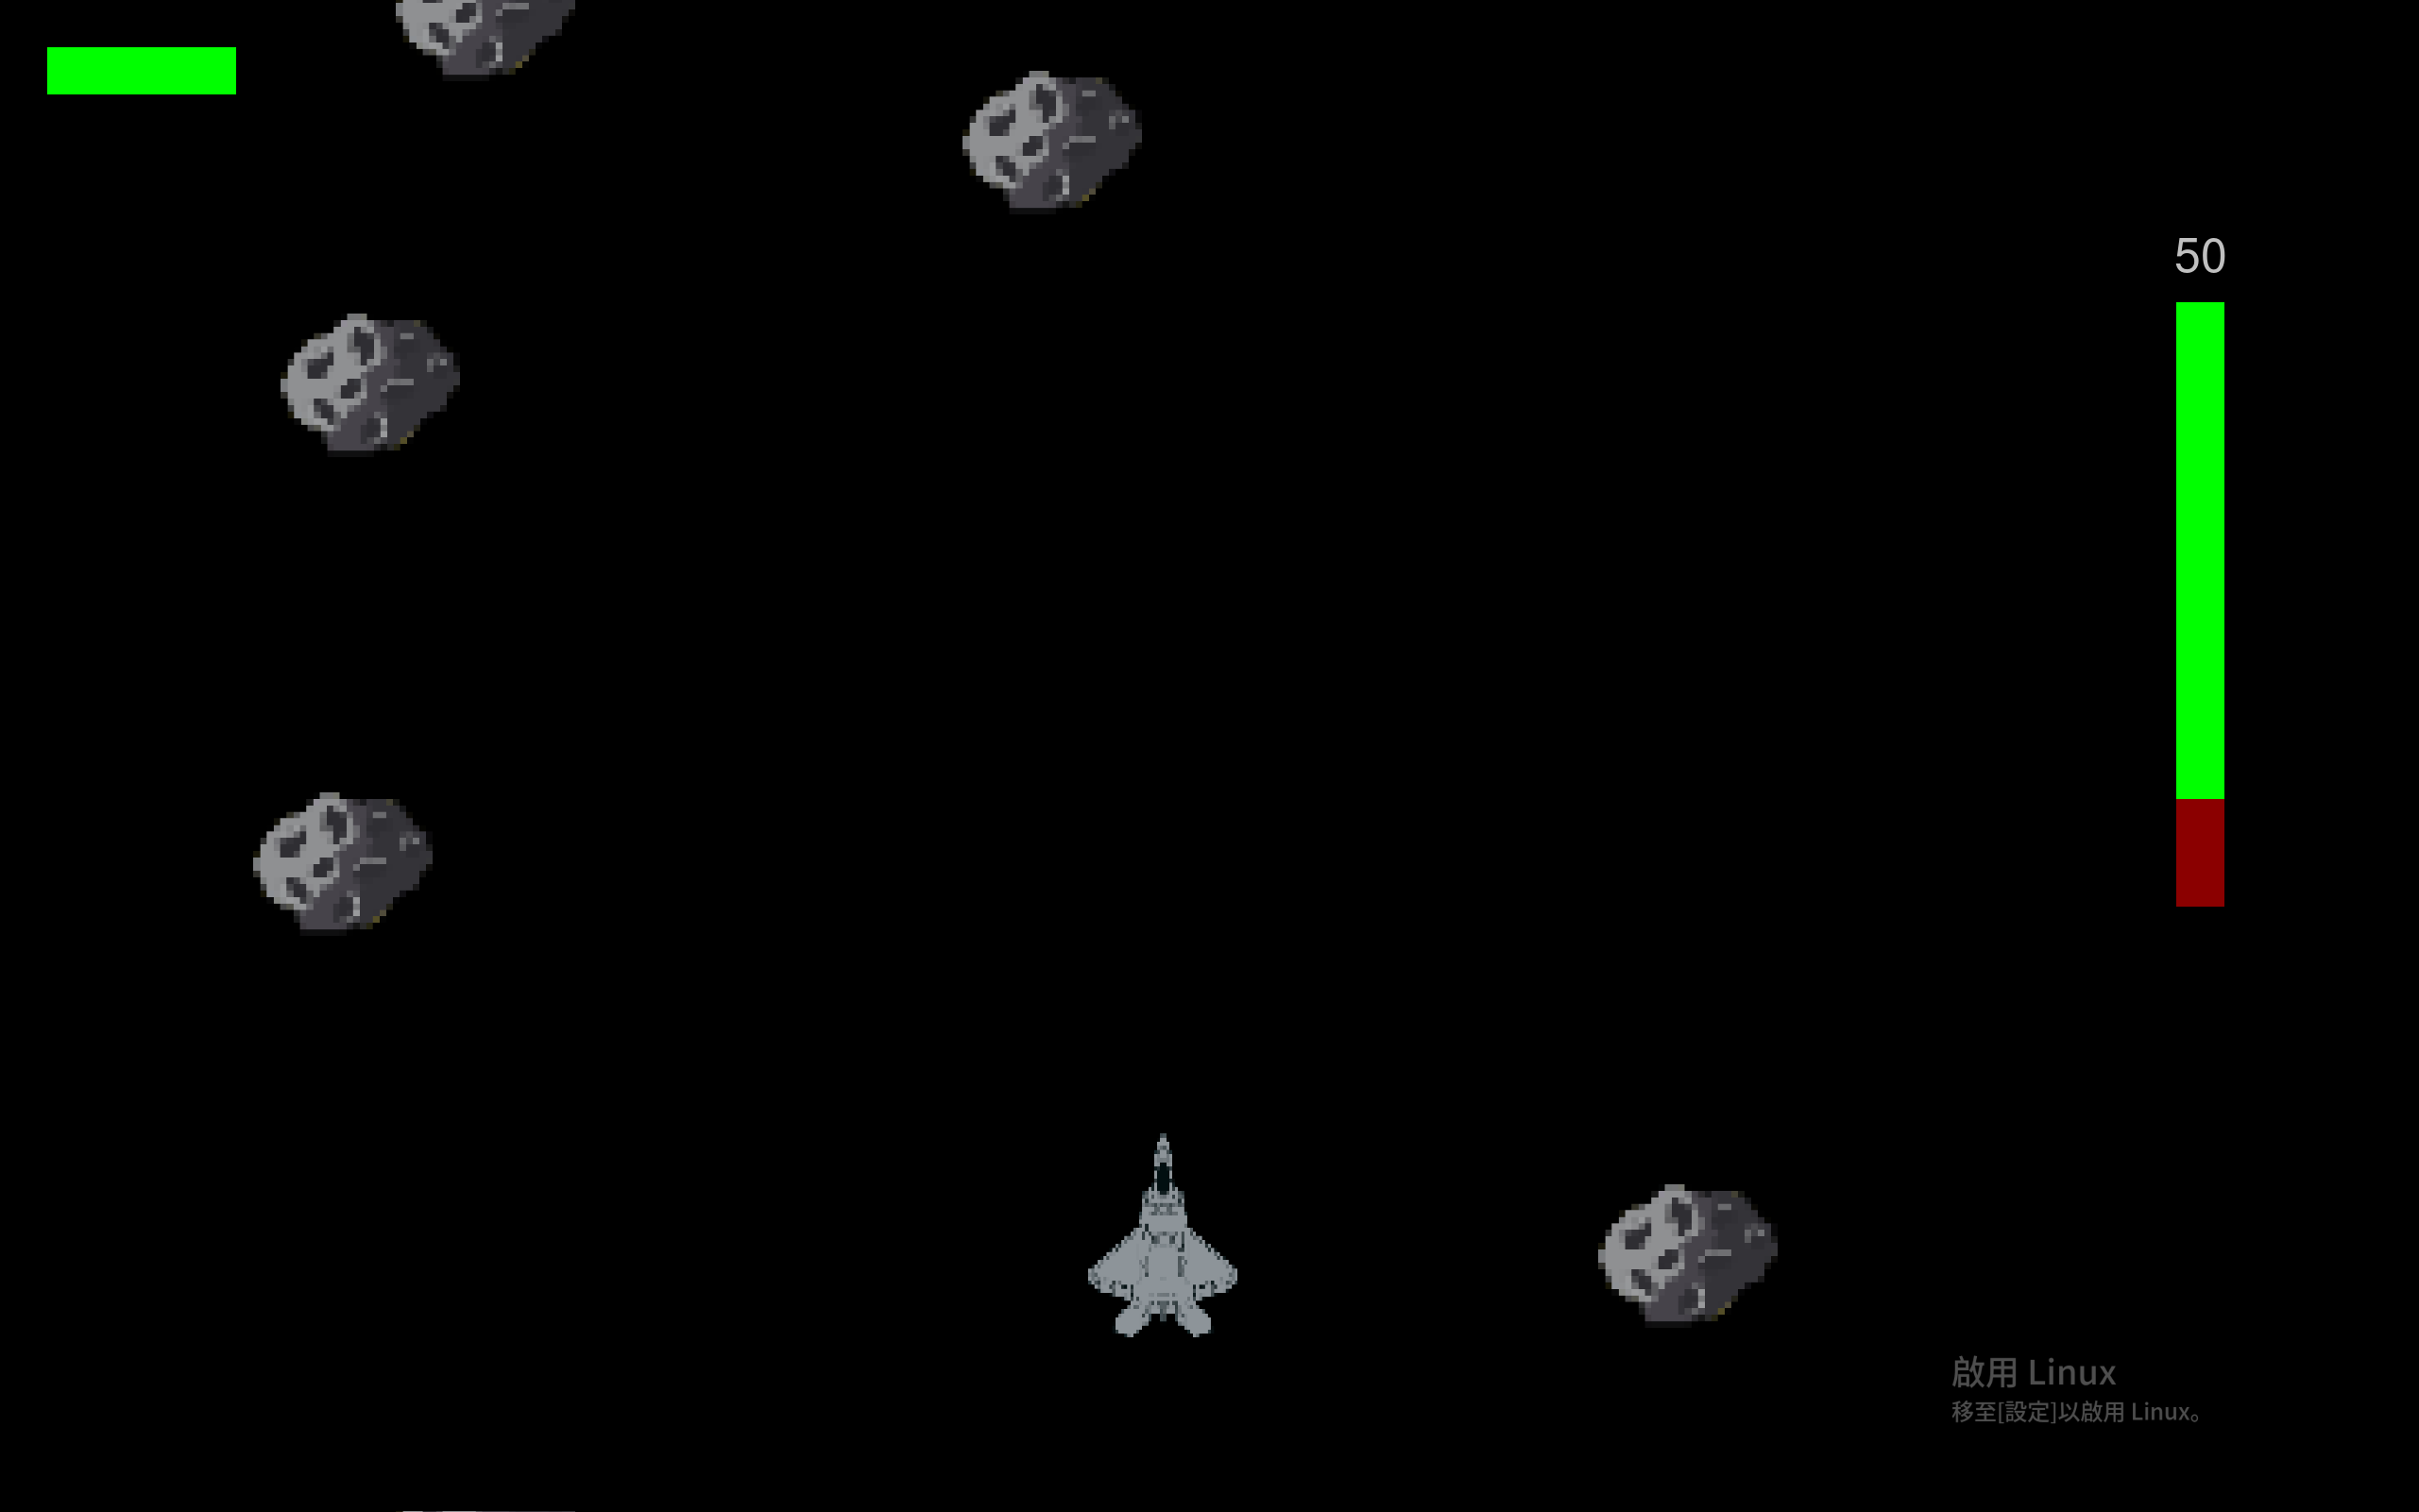
\includegraphics[width=\linewidth]{src/game.png}
\end{boxpar}

\begin{boxpar}{Dandelion}{反思與展望}
這次專題讓我第一次體驗到多人協作開發的真實樣貌。技術問題往往比溝通問題好解決。pygame 的 API 可以查文件，但組員之間對需求的理解落差，只能靠主動溝通來縮小。往後如果繼續參與多人開發，這件事是我會最先確認的環節。
\end{boxpar}

\end{large}
\end{document}
